\documentclass{article}

\usepackage[ngerman]{babel}
\usepackage{datetime}
\usepackage[a4paper,top=2cm,bottom=2cm,left=3cm,right=3cm,marginparwidth=1.75cm]{geometry}
\usepackage{amsmath}
\usepackage{graphicx}
\usepackage{float} % For forcing the position of elements
\usepackage[colorlinks=true, allcolors=blue]{hyperref}
\usepackage{fancyhdr} % For custom headers and footers
\usepackage{titlesec}  % For automatic new page at sections

% Set the Date Format
\newdateformat{myformat}{\THEDAY{ten }\monthname[\THEMONTH], \THEYEAR}

% Ensure a new page is started before every section
\newcommand{\sectionbreak}{\clearpage}
\newcommand{\thedate}{\today}

% Set up fancyhdr to customize the footer
\pagestyle{fancy}
\fancyhf{} % Clear default settings
\fancyfoot[C]{PREN Dokumentation - \thedate} % Add title and date to the center of the footer
\fancyfoot[R]{\thepage} % Page number on the right



\title{PREN Doku}
\author{Moritz Drillier \and Robin Venetz \and Benjamin Kuster \and Fabio Haueter \and Jonas Zimmermann \and Enya Senn}
\date{\thedate}

\begin{document}
\maketitle

\tableofcontents 

\begin{abstract}
Abstrakt
\end{abstract}

\section{Einleitung}
Das ist die Einleitung.
\section{Problemstellung}
Das ist die Problemstellung.
\section{Projektorganisation}

\subsection{Organigramm}

\subsection{Projektplan}
Hier ist ein Beispiel für eine Tabelle:

\begin{table}[H] % Use [H] to force the table position
    \centering
    \begin{tabular}{clr}
        1 & \date{\today} & 10 \\
        2 & Meilenstein 1 & 14 \\
        3 & Meilenstein 2  & 22 \\
        4 & Meilenstein 3  & 44 \\
        4 & Meilenstein 4  & 27 \\
    \end{tabular}
    \caption{Untertitel}
    \label{tab:my_label}
\end{table}

\subsection{Arbeitsmethodik}
According to \cite{sampleReference}, this is a relevant citation.


\subsection{Arbeitsmethodik}

\subsection{Risikomanagement \& Analyse}

\subsubsection{Risikomatrix}
\begin{figure}[H]
    \centering
    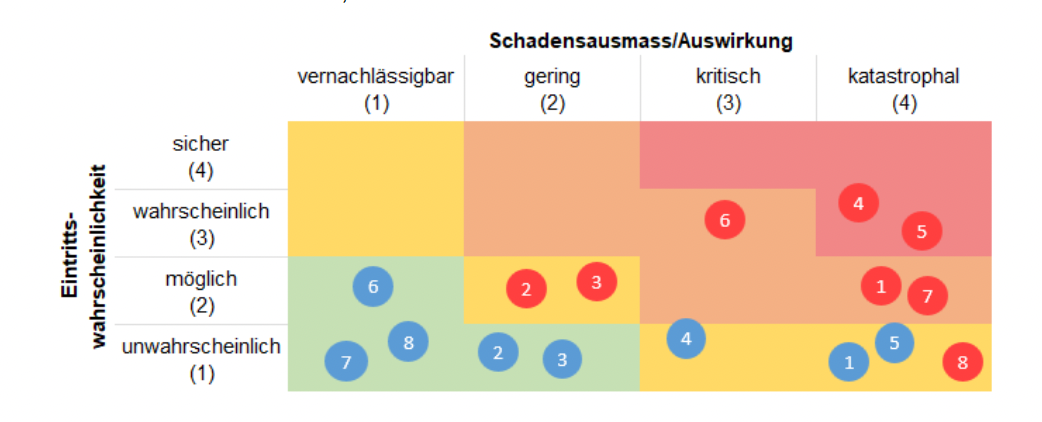
\includegraphics[width=0.8\linewidth]{Images/Risikomatrix.png}
    \caption{Enter Caption}
    \label{fig:enter-label}
\end{figure}

\subsection{Nachhaltigkeitsziele}
\subsection{Finanzen}

\newpage
\listoffigures % Abbildungsverzeichnis
\listoftables % Tabellenverzeichnis


\bibliographystyle{alpha}
\bibliography{Quellen}

\end{document}
